% !TEX root = ../my-thesis.tex
%
\chapter{Approach}
\label{sec:approach}

In this chapter the two alternatives to tackle the problem of ranking classification algorithms regarding properties of the data set based on past performance values are described in detail. First, the theoretical approach is presented. Then, implementation details are discussed.

\section{Theory}

Approach of ranking classifier implementations here realized by two concepts, regression-based and preference-based ranking, which will be explained in detail. Also predicting predictive accuracy here. Thus target function of the form $meta features^n \rightarrow classifiers^m$.
performance measure chosen predictive accuracy

% Theory of approach
Since the aim is to generate a ranking of classification algorithms, first, performance values of a number of classifiers are recorded on a few data sets. Then, meta features are computed for each data set. This is for training the ranking model. This generates a table that contains all necessary informatino for training both types of rankers. A ranking of the classifiers for a new instance is then achieved by computing the meta features for the data set and subsequently using it to query the underlying model. 

\begin{table}[h]
\centering
	\begin{tabularx}{\textwidth}{X | X | X | X | X | X | X | X}
		%\hline
		MF 1			& MF 2		& ... 	& MF n		& PV 1 		& PV 2 		&	...	&	PV k 		\\ \hline
		$v_{11}$		& $v_{12}$	& ...	& $v_{1n}$	& $p_{11}$	& $p_{12}$	& 	...	&	$p_{1k}$		\\ 
		$v_{21}$		& $v_{22}$	& ...	& $v_{2n}$	& $p_{21}$	& $p_{22}$	& 	...	&	$p_{2k}$		\\ 
		...			& ...		& ...	& ...		& ...		& ...		&	...	&	...			\\ 
		$v_{m1}$		& $v_{m2}$	& ... 	& $v_{mn}$	& $p_{2m}$	& $p_{m2}$	& 	...	&	$p_{mk}$			 
	\end{tabularx}
	\label{tab:performanceValues}
	\caption{This is a caption text.}
\end{table}

\subsection{Regression Based Ranking}
% How is the regression ranking done
One possibility to derive a ranking of classifiers from this information when given a new data set is to use regression models. The idea is to use separate regression models to predict a performance value for each classifier, and to then derive an ordering from these predictions. This is done by splitting the data set compiled beforehand into separate data sets that each contain all meta features for all data sets, but only the performance values of one classifier. The target feature on these individual data sets, the performance value of the classifier, is a numeric value, and thus a regression model can be trained on each of them. All regression models therefore try to learn the target function $meta features \rightarrow classifier performance value$ for their respective classifier. Hence for a query instance, after computing the meta features, these are fed into each regression model and the predicted performance value for each classifier is saved. In a second step, the classifiers are ordered according to the predictions.

\begin{table}[h]
\centering
\resizebox{\textwidth}{!}{%
	\begin{tabularx}{1.1\textwidth}{X | X | X | X}
		%\hline
		Meta Feature 1	& ... 	& Meta Feature n		& Performance Value 1	\\ \hline
		$v_{11}$			& ...	& $v_{1n}$			& $p_{11}$				\\ 
		$v_{21}$			& ...	& $v_{2n}$			& $p_{21}$				\\ 
		...				& ...	& ...				& ...					\\ 
		$v_{m1}$			& ... 	& $v_{mn}$			& $p_{m1}$				\\ \hline\hline
		Meta Feature 1	& ... 	& Meta Feature n		& Performance Value 2 	\\ \hline
		$v_{11}$			& ...	& $v_{1n}$			& $p_{12}$				\\ 
		$v_{21}$			& ...	& $v_{2n}$			& $p_{22}$				\\ 
		...				& ...	& ...				& ...					\\ 
		$v_{m1}$			& ... 	& $v_{mn}$			& $p_{m2}$					 
	\end{tabularx}
}	
\vspace{1em}
...
\vspace{1em}	
\resizebox{\textwidth}{!}{%
	\begin{tabularx}{1.1\textwidth}{X | X | X | X}
		%\hline
		Meta Feature 1	& ... 	& Meta Feature n		& Performance Value k 	\\ \hline
		$v_{11}$			& ...	& $v_{1n}$			& $p_{1k}$				\\ 
		$v_{21}$			& ...	& $v_{2n}$			& $p_{2k}$				\\ 
		...				& ...	& ...				& ...					\\ 
		$v_{m1}$			& ... 	& $v_{mn}$			& $p_{mk}$					 
	\end{tabularx}
}
	\label{tab:regressionTables}
	\caption{This is a caption text.}
\end{table}

\begin{figure}
\centering
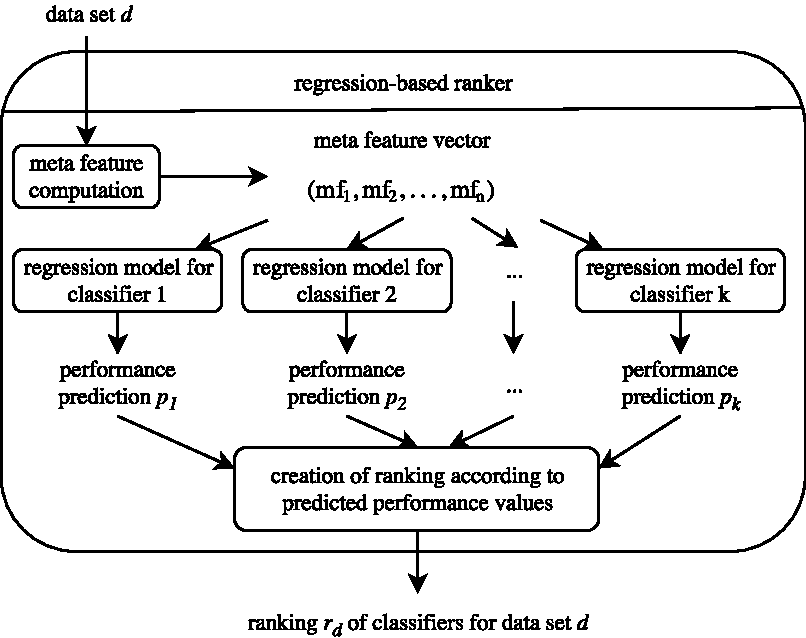
\includegraphics[scale=1]{gfx/regression_models.pdf}
\caption{A model of the regression based ranker}
\label{fig:regression_ranker_model}
\end{figure}

\subsection{Preference Based Ranking}
% How is the preference ranking done
The second possibility considered in this context is using preference learning to predict a ranking. Each instance of the data set generated beforehand contains meta feature information for the considered data set and performance values of all classifiers. Similarly to the regression alternative, the performance values can be converted to preference information by sorting the corresponding classifiers by their performance values. This leads to an ordering of classifiers associated with each instance, and implies that the preference learning task at hand is label ranking. In this case, there exists only one label ranking mode which is fed the computed meta data for a new data set and returns an ordering of classifiers. Thereby it attempts to learn the mapping from meta features to an ordering of classifiers directly.

\begin{table}[h]
\centering
	\begin{tabularx}{\textwidth}{X | X | X | X | X | X | X | X}
		%\hline
		MF 1				& MF 2				& ... 	& MF n				& PV 1 		& PV 2 		&	...	&	PV k 		\\ \hline
		$v_{11}$			& $v_{12}$			& ...	& $v_{1n}$			& $p_{11}$	& $p_{12}$	& 	...	&	$p_{1k}$		\\ 
		$v_{21}$			& $v_{22}$			& ...	& $v_{2n}$			& $p_{21}$	& $p_{22}$	& 	...	&	$p_{2k}$		\\
		...				& ...				& ...	& ...				& ...		& ...		&	...	&	...			\\
		$v_{m1}$			& $v_{m2}$			& ... 	& $v_{mn}$			& $p_{2m}$	& $p_{m2}$	& 	...	&	$p_{mk}$			 
	\end{tabularx}
	\label{tab:preferenceTable}
	\caption{This is a ranking}
\end{table}

\begin{figure}
\centering
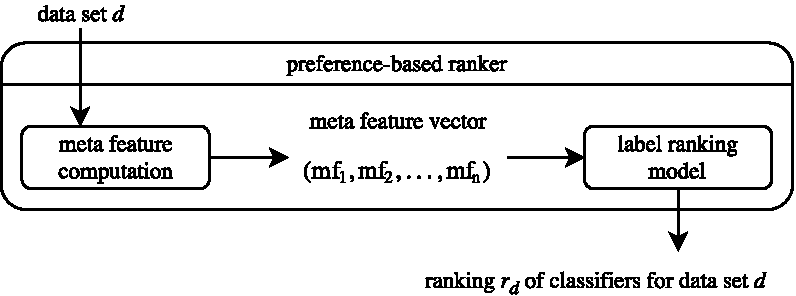
\includegraphics[scale=1]{gfx/label_ranking_model.pdf}
\caption{A model of the preference based ranker}
\label{fig:preference_ranker_model}
\end{figure}

\section{Implementation}
% regression based model - weka used

% preference learning
The jPL framework is a java framework for the evaluation of preference learning algorithms. It implements several tasks from the context of preference learning, including label ranking. 

% meta features - openML webapp
\cite{OpenML2013}
% Which meta features
As for the meta features, all meta features discussed in chapter \ref{sec:approach} where used. Initially, it was intended to download the computed meta features from OpenML, but since missing values for meta features ranged from roughly 25\% up to 89\% (except for a few simple meta features which were included for all data sets) it was decided to compute them anew. Meta features where calculated with the help of an implementation provided by OpenML \cite{openMLEvaluationEngine}. Two data sets, one including the downloaded meta features (for all 812 data sets) and one including the computed meta features (for the reduced set of 448 data sets) are thus included in the supplementary material. Since the meta data also includes probing, which is generally an expensive operation and furthermore does not aid in proving the point of a connection of properties of a data set and the performance of classifiers, additionally to the full meta features all evaluation measures where computed without using those meta features that use probing.

